% !TEX root = ../../main.tex

\section{Shaping in context}

In order to use an adsorbent in an industrial setting such as the beds and
columns common in PSA (pressure swing adsorption) and TSA (temperature 
swing adsorption) processes, a pelletized form of the material
is required.\cite{akhtarStructuringAdsorbentsCatalysts2014}

The kinetics of the adsorption process are generally improved by the multi-scale
pore size distribution afforded through shaping.
Capacity per mass of pellet is expected to decrease due to the
addition of a non-porous component, but the difference should be small and should not arise
due to effects such as pore blocking or pore filling with the binder material.
Furthermore, the densification effect is expected to lead to better performance on a volume basis.
Finally, binder addition should not influence the chemical properties of the adsorbent,
and preserve the original interactions with the adsorbate.
With a judicious choice of binding material, the resulting pellet
should outperform the powder.

\todo{shaping methods}

For carbons, binders such as pitch, polymers (CMC, PVA) or even non-porous carbon black
are commonly used~\cite{ohjiAdvancedProcessingManufacturing2008}.
Often, a combination of binders is used, each with a different task during the
pelletization process~\cite{bandoszActivatedCarbonSurfaces2006}.
The process itself consists of extrusion of the
particle-binder slurry and then hardening either through temperature, cross-linking
or chemical treatment. Other methods, such as spray-drying or granulation can similarly
be used~\cite{ruthvenPrinciplesAdsorptionAdsorption1984}.

For zeolites, inorganic binders are more prevalent, with silica, alumina and clay binders
commonly used in industry. It has been shown
\cite{whitingcuriouscasezeolite2016, MichelsEffectsBindersPerformance2014}
that the choice of binder can introduce large property variations, ranging from
loss of porosity and structure to the enhancement of the desired reactivity and selectivity
through changes in the acid site density or ion migration.

The shaping of MOFs has been attempted with a wide range of binders and methods.
Methods such as granulation, spray-drying or extrusion have all
been successfully employed to create MOF
pellets~\cite{kaskelChemistryMetalorganicFrameworks2016}.
Monoliths have also been shown to be an effective way for shaping purposes,
either through impregnation~\cite{ramos-fernandezMOFsMeetMonoliths2011} or through
support on alumina~\cite{aguadoFacileShapingImidazolatebased2010}.
Surprisingly, compression~\cite{bazer-bachiIndustrialUseMetalorganic2014} or even
simple air drying of MOF slurries~\cite{tianMechanicallyChemicallyRobust2015}
have also shown good results. Note that the ZIF-8 monolith prepared through the
latter method had a three times larger volumetric specific surface area than
the conventional powder.

The connection between MOF and binder is also of crucial importance for membranes.
The MOF-polymer interface has been shown~\cite{seminoMicroscopicModelMetal2016} to be
subject to a complex interplay of interactions between the organic chains and the
crystal surfaces. These effects can be striking enough to warrant further research
into MOF-polymer hybrids\cite{kitaoHybridizationMOFsPolymers2017}, with the aim of
combining the unique attributes of both materials.

Previous work from this group~\cite{chanutObservingEffectsShaping2016} has analysed the impact
of PVA shaping on a series of MOFs. It was shown that the binder did introduce
some specific effects, such as a protection effect on the reduction of \ce{Fe^3+} to
\ce{Fe^2+} in MIL-127(Fe), as well as a curious gating effect seen on butane adsorption
on MIL-100(Fe), likely due to polymer chains covering pore entrances. Otherwise, the
shaping imparted good performance to the shaped samples, with almost no capacity loss on
a mass basis. Unfortunately, the use of a polymer limited the activation temperature of the
samples to a maximum of \SI{150}{\degreeCelsius}.

In this work we have selected the same series of ``topical'' MOFs and have investigated the
influence of a different shaping method, namely the use of alumina binder, on their adsorption
properties.

The UiO-66(Zr) MOF and its derivatives are well known due to their stability, both in regards to
temperature and chemical compounds\cite{cavkaNewZirconiumInorganic2008}. It is composed of
Zr6-oxo clusters which are connected with benzene dicarboxilate (BDC) linkers to form
a face-centered cubic framework. It has shown promise~\cite{wiersumEvaluationUiO66GasBased2011}
in use for gas adsorption applications.

MIL-100(Fe) is a MOF which uses the benzene tricarboxilate (BTC) linker in conjunction
with trimeric iron (III) octahedral clusters.\cite{horcajadaSynthesisCatalyticProperties2007}
The framework assembles in hybrid supertetrahedra which leads to very large pore sizes.
The iron trimers are coordinated with
anions and have shown a propensity to partially reduce to a divalent \ce{Fe^2+} state, exposing
a naked metal site in the process.\cite{yoonControlledReducibilityMetalOrganic2010}

The last material, MIL-127(Fe), originally reported by~\citeauthor{liuAssemblyMetalOrganic2007} is
a MOF built from the same metal (III) octahedra trimers as MIL-100(Fe), but using the
3,3',5,5'-azobenzenetetracarboxylate (TazBz) linker, to produce a framework with the (soc)
topology. This material has shown promise~\cite{chevreauSynthesisBiocompatibleHighly2016}
for large scale synthesis. Furthermore, due to its alternating hydrophobic/hydrophilic
microporous systems, it has been shown to be of interest for multiple applications such
as catalysis or \ce{CO2} capture~\cite{chanutScreeningEffectWater2017}.

The structures of the three materials can be seen in \autoref{fgr:mofstructures}.

\begin{figure}[t]
	\centering
	\begin{subfigure}{0.3\textwidth}
		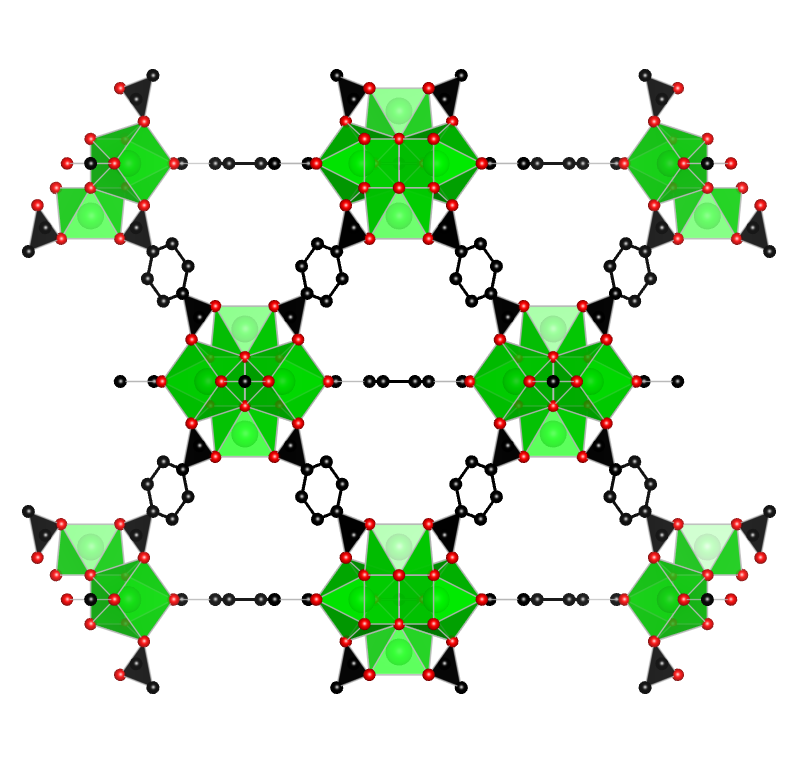
\includegraphics[width=\linewidth]{structure/uio66}
		\caption{UiO-66(Zr)}
	\end{subfigure}
	\begin{subfigure}{0.3\textwidth}
		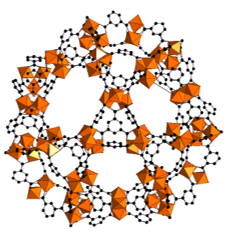
\includegraphics[width=\linewidth]{structure/mil100}
		\caption{MIL-100(Fe)}
	\end{subfigure}
	\begin{subfigure}{0.3\textwidth}
		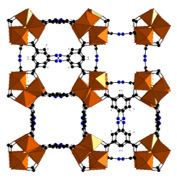
\includegraphics[width=\linewidth]{structure/mil127}
		\caption{MIL-127(Fe)}
	\end{subfigure}

	\caption{The unit structures of the investigated MOFs.
		The colour coding is as follows: Zr polyhedra in green,
		Fe octahedra in brown, C in black, O in red, N in blue.
		Hydrogen atoms are omitted for clarity.}
	\label{fgr:mofstructures}
\end{figure}